\chapter{Introdução}

Reconhecimento de gestos baseado em visão computacional é um assunto bastante pesquisado e já pode ser considerado popular nos dias de hoje, isto porque, a busca por mecanismos que tornem a interação entre homem e máquina mais intuitiva e natural é constante e vem aumentando com o lançamento de plataformas que auxiliam os desenvolvedores nos complexos algoritmos que envolvem essa área.
O lançamento do Kinect, da Microsoft \cite{kinect}, e da plataforma de desenvolvimento da Intel, chamada Intel Perceptual Computing \cite{intel},  ambas com câmeras de profundidade, vem popularizando o desenvolvimento de aplicativos e revolucionando o jeito que interagimos com os jogos e computadores. Em fevereiro de 2013 a Microsoft anunciou que um terço dos consoles Xbox 360 vendidos até o momento tinham o sensor Kinect, totalizando  uma venda de 24 milhões de sensores desde o lançamento do produto em novembro de 2010 \cite{kinect_sales}.

O uso de câmeras em carros e caminhões também tem aumentando nos últimos anos. Sistemas de segurança capazes de verificar se o motorista esta saindo indevidamente da faixa, se o veículo esta em rota de colisão com algum outro automóvel, pedestre ou objeto e câmeras noturnas, que proporcionam ao motorista uma visão extra quando a  estrada a frente esta escura, já são comuns em vários modelos de veículos. Em praticamente todos os modelos da Mercedes Benz, por exemplo, já é possível adquirir sistema de segurança desse tipo. Duas câmeras localizadas atrás do retrovisor e apontadas para a frente do veículo combinadas com um conjunto de radares fazem com que o motorista seja avisado caso aja risco de colisão, entre outras funcionalidades. Dependendo do caso o veículo pode atuar de forma autônoma e acionar os freios evitando uma colisão ou reduzindo a força do impacto \cite{mercedes_youtube, mercedes_safety}. 

Apesar do uso de câmeras para o lado externo do veículo já ser comum, ainda não é comum o uso dessas câmeras para interação do motorista com a grande quantidade de controles existentes nos carros. Sistemas de navegação, componentes de som e imagem como CD/DVD player, radio, televisão, celulares, computador de bordo, e ar condicionado são alguns exemplos de dispositivos que requerer uma constante interação e demandam uma grande quantidade de botões na região do console. Mesmo que os botões estejam agrupados em diferentes telas em um sistema multimédia, esse tipo de interação ainda exige uma grande atenção do motorista que precisa, na maioria dos casos, localizar visualmente o botão. Nem sempre também o uso dos botões ou da tela é confortável e ergométrico, podendo estar fora do alcance do motorista.

Uma maneira bastante natural de interagir com o veículo seria com voz e gestos. O sistema de voz já é bem comum hoje na maioria dos modelos de carros, mas são facilmente atrapalhados por barulhos internos e externo ao veículo e também interrompem o sistema de áudio, impossibilitando o seu uso caso, por exemplo, o sistema de viva voz estiver ativo. Portanto um sistema de gestos pode complementar a interface existente, dando mais opção aos usuários na hora enviar comandos para o veículo.

Nesse sistema gestual de interação do motorista com o veículo, entende-se poses e gestos como sendo movimentos ou poses executados pela mão direta do motorista dentro do campo de visão de uma câmera instalada no teto do carro.
O estudo desse trabalho, portanto, é focado na analise de um sistema capaz de caracterizar as poses de mão para que possam ser classificadas e usadas em um sistema de interface de usuário. Um sistema em tempo real capaz de reconhecer poses de mão e gestos que permita o motorista interagir com o veículo de forma intuitiva e eficaz. Na figura \ref{fig:visao_aplicacao} tem-se um exemplo de como seria uma pose de mão aberta dentro de um ambiente automotivo.

\begin{figure}[ht!]
	\centering
	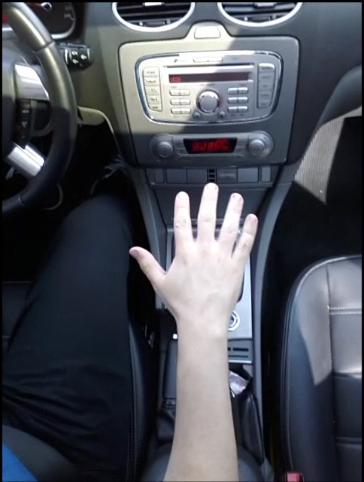
\includegraphics[width=0.3\textwidth]{image/exemplo_visao_aplicacao.png}
	\caption{Exemplo do uso de poses em um ambiente automotivo}
	\label{fig:visao_aplicacao}
\end{figure}

\section{Objetivo}

O objetivo do trabalho é encontrar em uma imagem obtida no interior do veículo, do ponto de vista do teto e nas mais variadas condições de luminosidade, uma região de interesse com uma alta probabilidade de se ter uma pose de mão. A proposta é estudar o desempenho do histograma de orientações de gradientes (HOG - Histogram of Oriented Gradients) nessas condições e analisar o comportamento das variações dos parâmetros na aplicação e a influencia das variáveis do ambiente (mudança de veículo, de motorista e de luminosidade) no algoritmo.
Um balanço entre performance e processamento deve ser levado em consideração, já que o trabalho computacional deve ser reduzido ao máximo para aplicações automotivas.

Um dos primeiros passos no processamento de uma imagem, com o objetivo de se identificar uma pose, é encontrar a região de interesse. Essa região é uma sub imagem onde a mão aparece com mais evidencia, eliminando as partes da cena que não são de interesse. Com o escopo reduzido, fica mais robusto aplicar outros algoritmos para a detecção da pose.

A escolha do HOG como descritor para as poses de mão se da por conta da sua grande robustez contra variações de luminosidade. O HOG foi proposto por \citeonline{dalal2005histograms} que encontraram o melhor conjunto de parâmetros para a representação de seres humanos em diversas situações e poses diferentes. 

O descritor poderia ser usado de duas maneiras diferentes: como um pre classificador para encontrar as regiões mais prováveis de se ter uma mão e assim limitar a imagem em algumas regiões de interesse aonde um segundo algoritmo seria aplicado, nesse caso não seria trabalho do HOG dizer qual é a pose, mas sim se é uma mão ou não, ou no máximo classificar a pose em algum grupo de poses (como feito em \cite{jiang2012robust}). Mas o HOG poderia ser usado também para dizer qual pose é, sem a necessidade de nenhum algoritmo secundário.
Visando que temos duas aplicações para o HOG, é possível que teremos duas configurações diferentes e portanto essas variações devem entrar no escopo desse trabalho.

Trabalha-se portanto com a hipótese de que o HOG pode ser parametrizado para encontrar poses de mão. E o conjunto original de parâmetros podem ser modificados para melhor de adequar à aplicação proposta.

\section{Justificativa}

A função principal do motorista deve ser sempre o controle do veículo. Distrações, como operar o rádio ou a central multimédia são exemplos constantes de cause de acidentes. Portanto apenas alguns poucos e curtos momentos podem ser usados para interagir com os comandos do veículo. Em estudos de usabilidade, o controle gestual provou ser mais intuitivo, efetivo \cite{zobl2001usability} e distrair menos do que o uso habitual de botões \cite{geiger2001intermodal}. Por esse motivo, um estudo sobre técnicas para atingir esse objetivo é justificável.

As condições gerais dentro do automóvel inclui uma grande variação de iluminação, mudança de usuário (cor de pele, braço com ou sem vestimentas e vestimentas de cores e estampas diferentes) e fundos não uniformes. Além disso, a aceitação do usuário é um item bastante importante, portanto coisas como uma iluminação artificial visível, restrição de vestimentas e calibração extensiva não pode ser tolerados. Tento isso em mente, alguns critérios e requisitos para o sistema podem ser estabelecidos:

\begin{itemize}
\item robustez contra ambientes ruidosos
\item iluminação invisível
\item independente de usuário
\item sem calibração ou treinamento pelo usuário
\item pequeno e compreensível conjunto de gestos
\item reação do sistema com o mínimo de latência
\end{itemize}

O estudo de \citeonline{dalal2005histograms} sobre histogramas de orientação de gradientes, aplicado à detecção de humanos variando cada parâmetro do cálculo dos histogramas e encontrando um conjunto de parâmetros que melhor servia para reconhecimento de humanos, virou referência para todos os estudos posteriores na área. Em seu texto ele diz que o uso de histogramas orientados tem muitos precursores \cite{freeman1995orientation, freeman1996computer}, mas que apenas atingiu a maturidade quando combinado com histogramas locais e normalização proposto pela Lowes Scale Invariant Feature Transformation (SIFT) \cite{lowe2004distinctive}. A conclusão que ele chegou foi que usando histogramas de gradientes locais normalizados, similar ao SIFT, em um grade com sobreposição tem ótimos resultados para detecção de humanos, reduzindo falsos positivos em mais de uma ordem de magnitude comparado com Haar wavelets.

\section{Metodologia}

A primeira etapa do projeto é a captura das poses, a pesquisa literária mostra \cite{zobl2004gesture, akyol2000gesture} que o uso de uma câmera infravermelha simples já é adequado para o problema, onde o ambiente é iluminado por infravermelho de curta distância (950nm). A câmera ainda possui um filtro de luz, permitindo apenas que a luz infravermelha seja capturada. Apesar de existir câmeras mais sofisticadas de alta resolução e tecnologias que permitem calcular a distância entre a câmera e o objeto, optou-se por usar a webcam simples por ser mais compatível com os padrões de mercado automotivo. No momento que esse texto foi escrito, as câmeras de profundidade, por exemplo, ainda possuem um preço proibitivo e a quantidade de processamento é bastante limitada em um ambiente embarcado.

As imagens de poses e os vídeos dos gestos serão obtidos em  dois ambientes distintos. Primeiro em um ambiente controlado com fundo homogêneo de cor preta e em uma sala totalmente escura (essa base de dados será usada como referência para os algoritmos implementados). O outro será obtido no interior de um veículo, tanto de dia como de noite. A captura das imagens no interior do veículo é obtida variando tanto o motorista quanto o veículo. Também será usado outras bases de dados que não em veículos para comparar a performance do algoritmo nas mais diversas situações.

Próximo passo é a implementação do algoritmo HOG para depois variar os parâmetros e analisar com o melhor conjunto. Pode-se usar como referência a implementação feito pelo MATLAB, que usou os parâmetros de \citeonline{dalal2005histograms} em sua implementação e ainda permite um certo grau de parametrização.

Com relação às poses, vamos analisar a performance de 11 poses diferentes e analisar quais são as poses mais adequadas e que melhor se destacam para o uso em nossa aplicação. Para ter uma noção visual do quanto as poses são diferentes entre si, vamos reduzir as dimensões do vetor de características gerado pelo algoritmo para apenas 3 dimensões. Usando o PCA podemos fazer essa redução e encontrar os 3 auto vetores e auto valores que melhor caracterizam nossas imagens e com isso conseguiremos um gráfico de três dimensões e ter uma perspectiva do quando os gestos estão agrupados entre si.

\section{Organização da dissertação}

Em construção.

